% Para compilar correr: "make" e dpois "make clean"
\documentclass{report}
\usepackage[T1]{fontenc} % Fontes T1
\usepackage[utf8]{inputenc} % Input UTF8
\usepackage[backend=biber, style=ieee]{biblatex} % para usar bibliografia
\usepackage{csquotes}
\usepackage[portuguese]{babel} %Usar língua portuguesa
\usepackage{blindtext} % Gerar texto automaticamente
\usepackage[printonlyused]{acronym}
\usepackage{hyperref} % para autoref
\usepackage{graphicx}

\bibliography{bibliografia}


\begin{document}
%%
% Definições
%
\def\titulo{PROJETO 2}
\def\data{14/07/2021}
\def\autores{Gonçalo Silva, Samuel Teixeira, Pompeu Costa, Hugo Hadden}
\def\autorescontactos{(103244) goncalolsilva@ua.pt, (103325) samuelsteixeira@ua.pt,\\
 (103294) pompeu@ua.pt,(98449) hugohadden@ua.pt}
\def\versao{VERSAO FINAL}
\def\departamento{Departamento de Eletrónica, Telecomunicações e
Informática}
\def\empresa{Universidade de Aveiro}
\def\logotipo{ua.pdf}
%
%%%%%% CAPA %%%%%%
%
\renewcommand{\contentsname}{Índice}
\begin{titlepage}

\begin{center}
%
\vspace*{50mm}
%
{\Huge \titulo}\\ 
%
\vspace{10mm}
%
{\Large \empresa}\\
%
\vspace{10mm}
%
{\LARGE \autores}\\ 
%
\vspace{30mm}
%
\begin{figure}[h]
\center
\includegraphics{\logotipo}
\end{figure}
%
\vspace{30mm}
\end{center}
%
\begin{flushright}
\versao
\end{flushright}
\end{titlepage}

%%  Página de Título %%
\title{%
{\Huge\textbf{\titulo}}\\
{\Large \departamento\\ \empresa}
}
%
\author{%
    \autores \\
    \autorescontactos
}
%
\date{\data}
%
\maketitle

\pagenumbering{roman}

%%%%%%%%%%%%%%%%%%%%%%%%%%%%%%%% RESUMO %%%%%%%%%%%%%%%%%%%%%%%%%%%%%%%%
\begin{abstract}
Este projeto foi realizado no âmbito da cadeira \ac{labi} do 1º ano do \ac{miect}. 
Consiste na criação de um sistema que permita criar músicas através da composição 
de pedaços/ excertos de música. Para além disso, também tivemos de fazer
este mesmo relatório em que explicamos o projeto: objetivo, motivação, a
metodologia utilizada, resultados, análise e conclusões.
Na metodologia, será relatado em pormenor o código feito para construir este projeto
, bem como o modo de funcionamento, testagem e comandos git feitos para tal.
Nos resultados, será mostrado o fruto de todo o nosso código que é a aplicação web a funcioanr.
Por fim, nas conclusões, retira-se o que se alcançou com este projeto, o que aprendemos,
o quão útil este projeto é para compreendermos esta matéria da cadeira de LABI e o 
quão interessante foi realizá-lo.
\end{abstract}

%%%%%%%%%%%%%%%%%%%%%%%%%%%%%%%% Agradecimentos %%%%%%%%%%%%%%%%%%%%%%%%%%%%%%%%
% Segundo glisc deveria aparecer após conclusão...
\renewcommand{\abstractname}{Agradecimentos}
\begin{abstract}
Queremos agradecer a todos os professores da cadeira de \ac{labi} por nos terem
dado um trabalho interessante, que nos ajudou a compreender os conceitos
lecionados nas aulas.
\end{abstract}


\tableofcontents
% \listoftables     % descomentar se necessário
% \listoffigures    % descomentar se necessário


%%%%%%%%%%%%%%%%%%%%%%%%%%%%%%%
\clearpage
\pagenumbering{arabic}

%%%%%%%%%%%%%%%%%%%%%%%%%%%%%%%% INTRODUÇÃO %%%%%%%%%%%%%%%%%%%%%%%%%%%%%%%%%

\chapter{Introdução}
\label{chap.introducao}

O objetivo deste trabalho é criar uma aplicação web que permita criar músicas através da 
composição de excertos. A Interface web, tem três páginas, na primeira são 
listadas as músicas existentes, na segunda os excertos e na terceira, um gerador de 
músicas, que permita ao utilizador criar a sua própria música, baseada nos excertos 
disponíveis. Além disso, nas duas primeiras páginas, é possível o utilizador visualizar a
informação acerca de cada música/ excerto, sendo até possível ouvi-lo.

Este documento está dividido em quatro capítulos.
Depois desta introdução,
no \autoref{chap.metodologia} é apresentada a metodologia seguida,
no \autoref{chap.resultados} são apresentados os resultados obtidos,
sendo estes discutidos no \autoref{chap.analise}.
Finalmente, no \autoref{chap.conclusao} são apresentadas
as conclusões do trabalho.

%%%%%%%%%%%%%%%%%%%%%%%%%%%%%%%%% METODOLOGIA %%%%%%%%%%%%%%%%%%%%%%%%%%%%%%%%%

\chapter{Metodologia}
\label{chap.metodologia}
Como o título sugere, neste capítulo vamos mostrar e explicar os métodos e ferramentas 
que usámos para completar este projeto. 

%%%%%%%%%%%%%%%%%%%%%%%%%%%%%%% MET: GERADOR DE MÚSICAS %%%%%%%%%%%%%%%%%%%%%%%%%%%%%%%
\section{Gerador de Músicas}
\label{sec:songEngine}
Nesta secção será apresentada a metodologia do Gerador de Músicas, ficheiro songEngine.py.

\subsection{Função readSong}
\label{ssec:readSong}
A função readSong, como se poder fer na \textbf{\autoref{fig:readSong}}, recebe como parâmetros um ficheiro .wav e devolve a informação acerca do mesmo,
no formato wave\_params, que corresponde a uma lista a cujos índices guardam a informação da seguinte forma:
\begin{itemize}
    \item \textbf{'0'} - Número de canais do ficheiro (nchannels);
    \item \textbf{'1'} - Largura da sample em bytes (sampwidth);
    \item \textbf{'2'} - Frequência da sample em bytes (Framerate);
    \item \textbf{'3'} - Número de frames de audio (nframes);
    \item \textbf{'4'} - Tipo de compressão (comptype)
    \item \textbf{'5'} - Idêntico ao ponto anterior, mas um nome, geralmente 'not compressed' (compname)
\end{itemize}

\begin{figure}[!h]
\center 
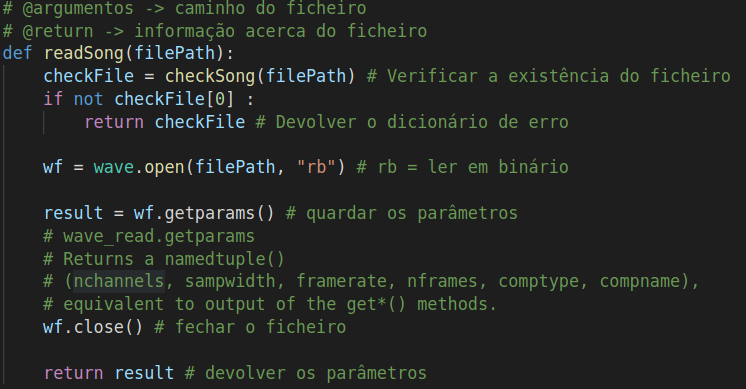
\includegraphics[height=160pt]{img/readSong.png}
\caption{Código da função readSong}
\label{fig:readSong}
\end{figure}

\subsection{Função checkSong}
\label{ssec:checkSong}
Esta função (\textbf{\autoref{fig:checkSong}}) recebe um caminho de um ficheiro e devolve se este existe, em formato de lista. De acordo com o caminho fornecido, 
as possíveis respostas da função, são:
\begin{itemize}
    \item \textbf{'Ficheiro'} - [True, "success"];
    \item \textbf{'Diretório'} - [False, "The provided path is a directory"];
    \item \textbf{'Não encontrado'} - [False, "The provided path doesn't exists"];
\end{itemize}

\begin{figure}[!h]
\center 
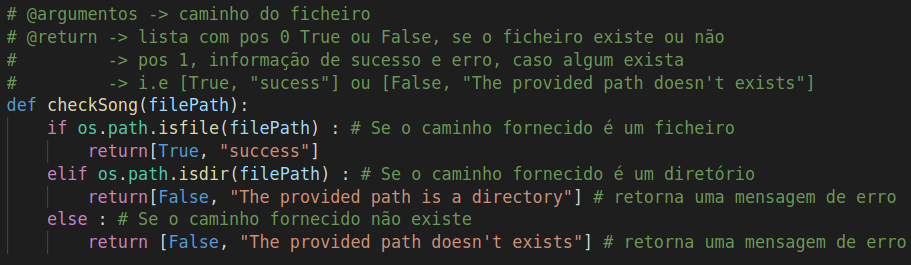
\includegraphics[height=100pt]{img/checkSong.png}
\caption{Código da função checkSong}
\label{fig:checkSong}
\end{figure}

\subsection{Função durationSong}
\label{ssec:durationSong}
A função durationSong aceita como parâmetros um caminho de um ficheiro e devolve a sua duração em segundos. Ela efetua este
cálculo com a fórmula \(waveFile.nframes / float(waveFile.framerate)\) (\textbf{\autoref{fig:durationSong}}).

\begin{figure}[!h]
\center 
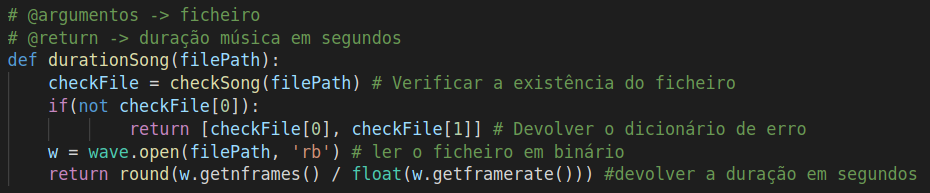
\includegraphics[width=330pt]{img/durationSong.png}
\caption{Código da função durationSong}
\label{fig:durationSong}
\end{figure}

\subsection{Função calculateFramerate}
\label{ssec:calculateFramerate}
Na \textbf{\autoref{fig:calculateFramerate}} podemos ver a função calculateFramerate que, tendo sido fornecidos os \ac{bpm},
devolve a framerate pretendida para ajustar na música. utilizando a fórmula \(bpm * 44100 / 60\)

\begin{figure}[!h]
\center 
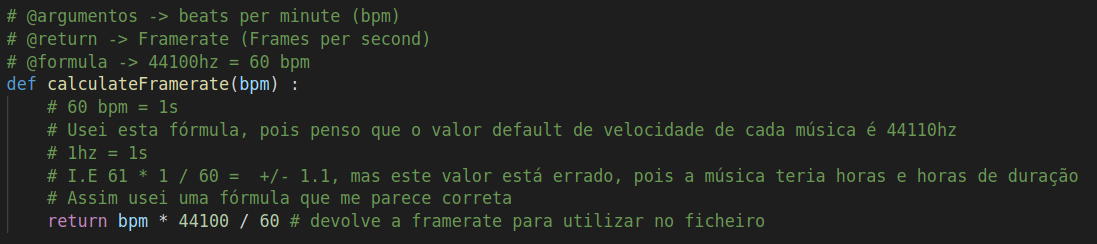
\includegraphics[width=330pt]{img/calculateFramerate.png}
\caption{Código da função calculateFramerate}
\label{fig:calculateFramerate}
\end{figure}

\subsection{Funções fadeInSong e fadeOutSong}
\label{ssec:FadeinFadeout}
A \textbf{\autoref{fig:FadeinFadeout}} mostra-nos as funções fadeInSong e fadeOutSong que aplicam os efeitos Fade In e Fade Out 
à música, respetivamente. Para isso, aceita como parâmetros a música, sample rate (ou framerate) e a duração do efeito.

\begin{figure}[!h]
\center 
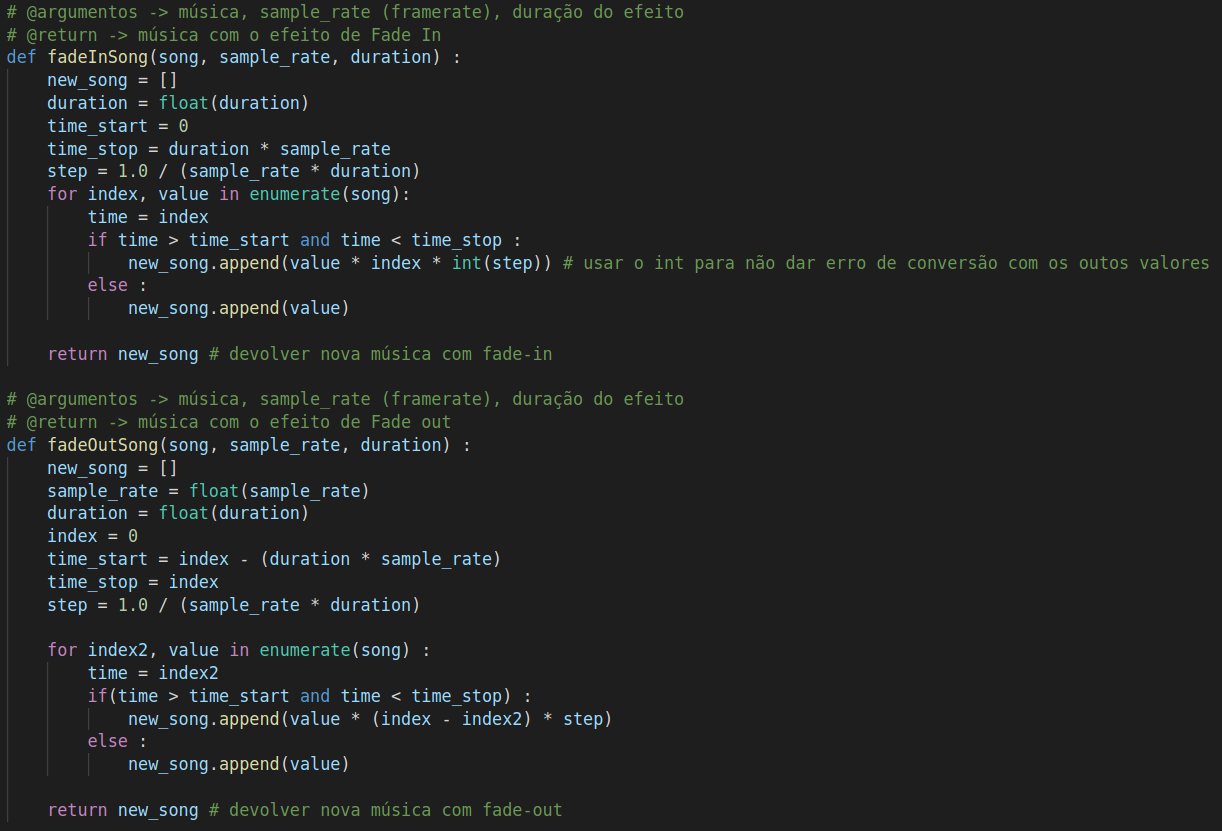
\includegraphics[width=330pt]{img/fadeInFadeOut.png}
\caption{Código das funções fadeInSong e fadeOutSong}
\label{fig:FadeinFadeout}
\end{figure}

\subsection{Função reverseSong}
\label{ssec:reverseSong}
Na \textbf{\autoref{fig:reverseSong}} está presente a função reverseSong, que aceita uma música e a inverte. Ou seja, 
o ínicio da música passa a ser o fim e o fim o ínicio.

\begin{figure}[!h]
\center 
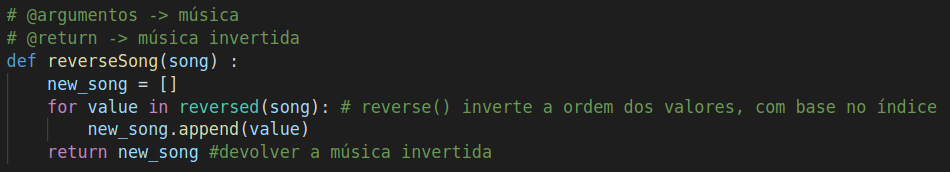
\includegraphics[width=330pt]{img/reverseSong.png}
\caption{Código da função reverseSong}
\label{fig:reverseSong}
\end{figure}

\subsection{Função volumeSong}
\label{ssec:volumeSong}
A \textbf{\autoref{fig:volumeSong}} mostra a função volumeSong, que ajusta o volume da música, tendo em conta o novo volume 
fornecido pelo utilizador. Para ajustar o volume da música, a mesma é multiplicada pelo novo volume, em que 1, corresponde ao 
valor atual, sem alteração, 0.5 diminui o volume e 2 multiplica o volume.

\begin{figure}[!h]
\center 
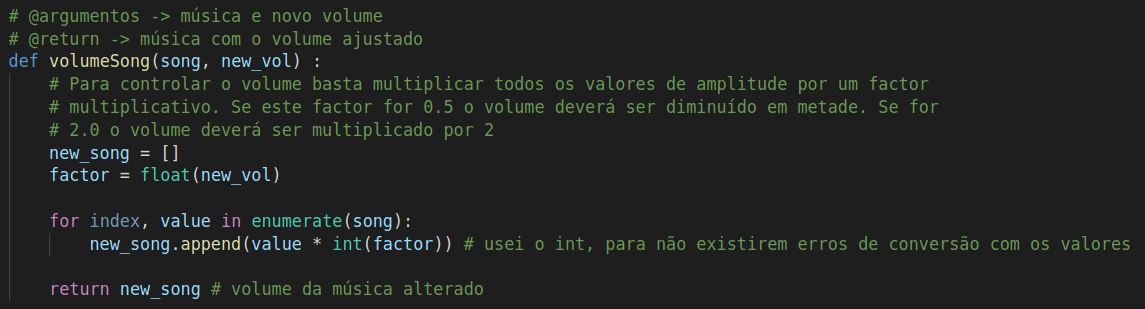
\includegraphics[width=330pt]{img/volumeSong.png}
\caption{Código da função reverseSong}
\label{fig:volumeSong}
\end{figure}

\subsection{Função normalizeSong}
\label{ssec:normalizeSong}
Na \textbf{\autoref{fig:normalizeSong}} está presente a função normalizeSong, que aceita uma música e a devolve com o som 
normalizado/ regulado, fazendo uso da \nameref{ssec:volumeSong}. No entanto, esta função não funciona na aplicação final, 
devido a erros de conversão no código.

\begin{figure}[!h]
\center 
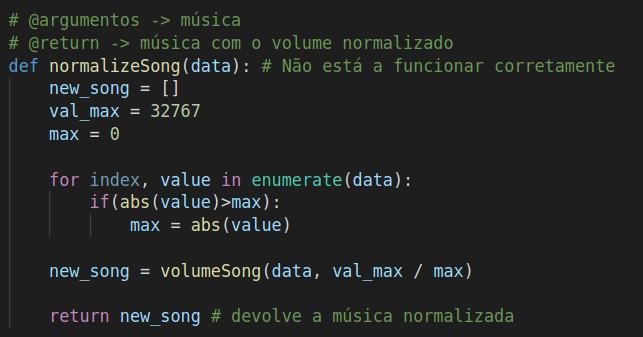
\includegraphics[width=330pt]{img/normalizeSong.png}
\caption{Código da função normalizeSong}
\label{fig:normalizeSong}
\end{figure}

\subsection{Função maskSong}
\label{ssec:maskSong}
Na \textbf{\autoref{fig:maskSong}} está presente a função maskSong, que permite aplicar uma máscara à música. Existem três
máscaras disponíveis:
\begin{itemize}
    \item \textbf{'silence'} - Permite silenciar a música;
    \item \textbf{'noise'} - Acrescenta ruído à música;
    \item \textbf{'tone'} - Tonifica a música;
\end{itemize}
Depois de aplicados os efeitos, a função irá retornar a música com os efeitos aplicados.

\begin{figure}[!h]
\center 
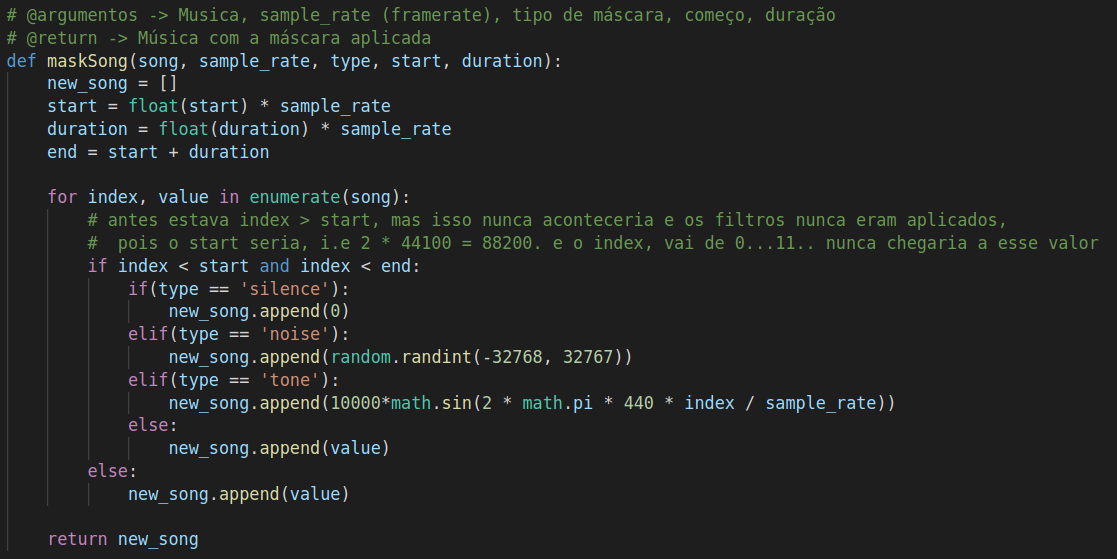
\includegraphics[width=330pt]{img/maskSong.png}
\caption{Código da função maskSong}
\label{fig:maskSong}
\end{figure}

\subsection{Função modulateSong}
\label{ssec:modulateSong}
Na \textbf{\autoref{fig:modulateSong}} está presente a função modulateSong que aplica uma modulação à música, utilizando 
uma sample rate e frequência fornecida pelo utilizador. No entanto, esta função não funciona na aplicação final, 
devido a erros de conversão no código.

\begin{figure}[!h]
\center 
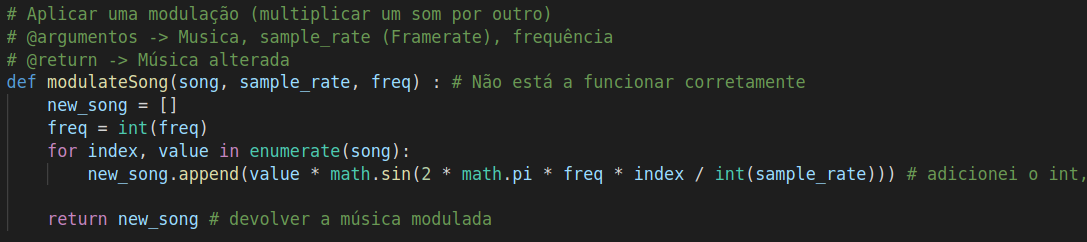
\includegraphics[width=330pt]{img/modulateSong.png}
\caption{Código da função modulateSong}
\label{fig:modulateSong}
\end{figure}

\subsection{Função delaySong}
\label{ssec:delaySong}
A \textbf{\autoref{fig:delaySong}} mostra a função delaySong que permite aplicar um delay/ atraso na música, com o início e
duração fornecidos pelo utilizador, devolvendo a música com o delay aplicado.

\begin{figure}[!h]
\center 
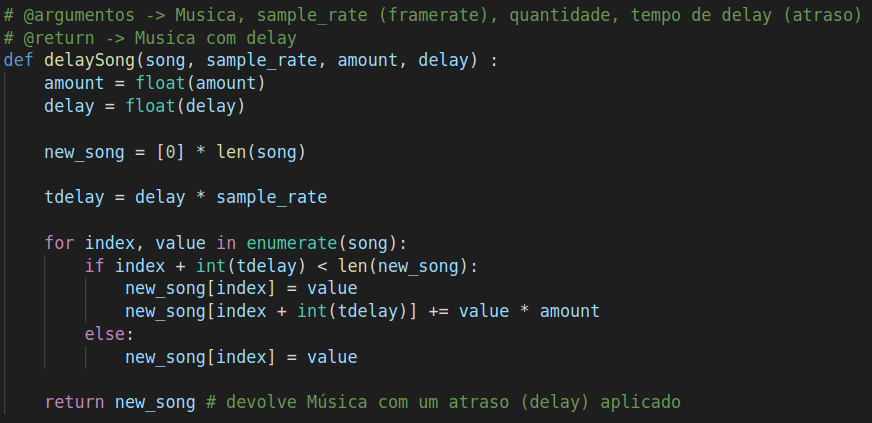
\includegraphics[width=330pt]{img/delaySong.png}
\caption{Código da função delaySong}
\label{fig:delaySong}
\end{figure}

\subsection{Função effectsSong}
\label{ssec:effectsSong}
A \textbf{\autoref{fig:effectsSong}} mostra a função effectsSong, que permite escolher qual o efeito a aplicar a uma música e
os parâmetros que serão aplicados.

\begin{figure}[!h]
\center 
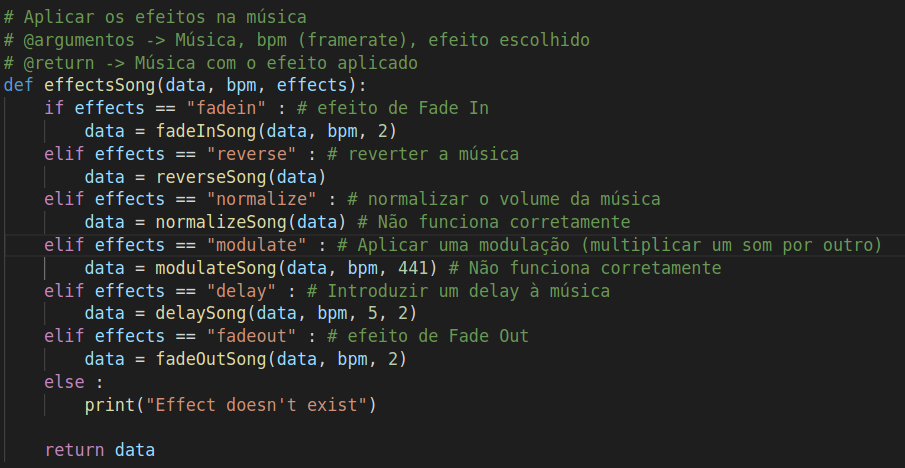
\includegraphics[width=330pt]{img/effectsSong.png}
\caption{Código da função effectsSong}
\label{fig:effectsSong}
\end{figure}

\subsection{Função createSong}
\label{ssec:createSong}
A \textbf{\autoref{fig:createSong}} mostra a função createSong, onde um dicionário \ac{json} é fornecido como argumento, para criar
uma música e depois de os campos deste dicionário serem testados, a função gera uma música com os valores fornecidos. Fazendo 
uso das funções mencionadas acima, a função também pode aplicar efeitos e alterar parâmetros para combinar vários excertos
numa só música, que é devolvida ao utilizador. No entanto, se alguma das verificações ou processos não for bem sucedido, a
função devolve uma mensagem de erro em formato de list: [False, "erro"].

\begin{figure}[!h]
\center 
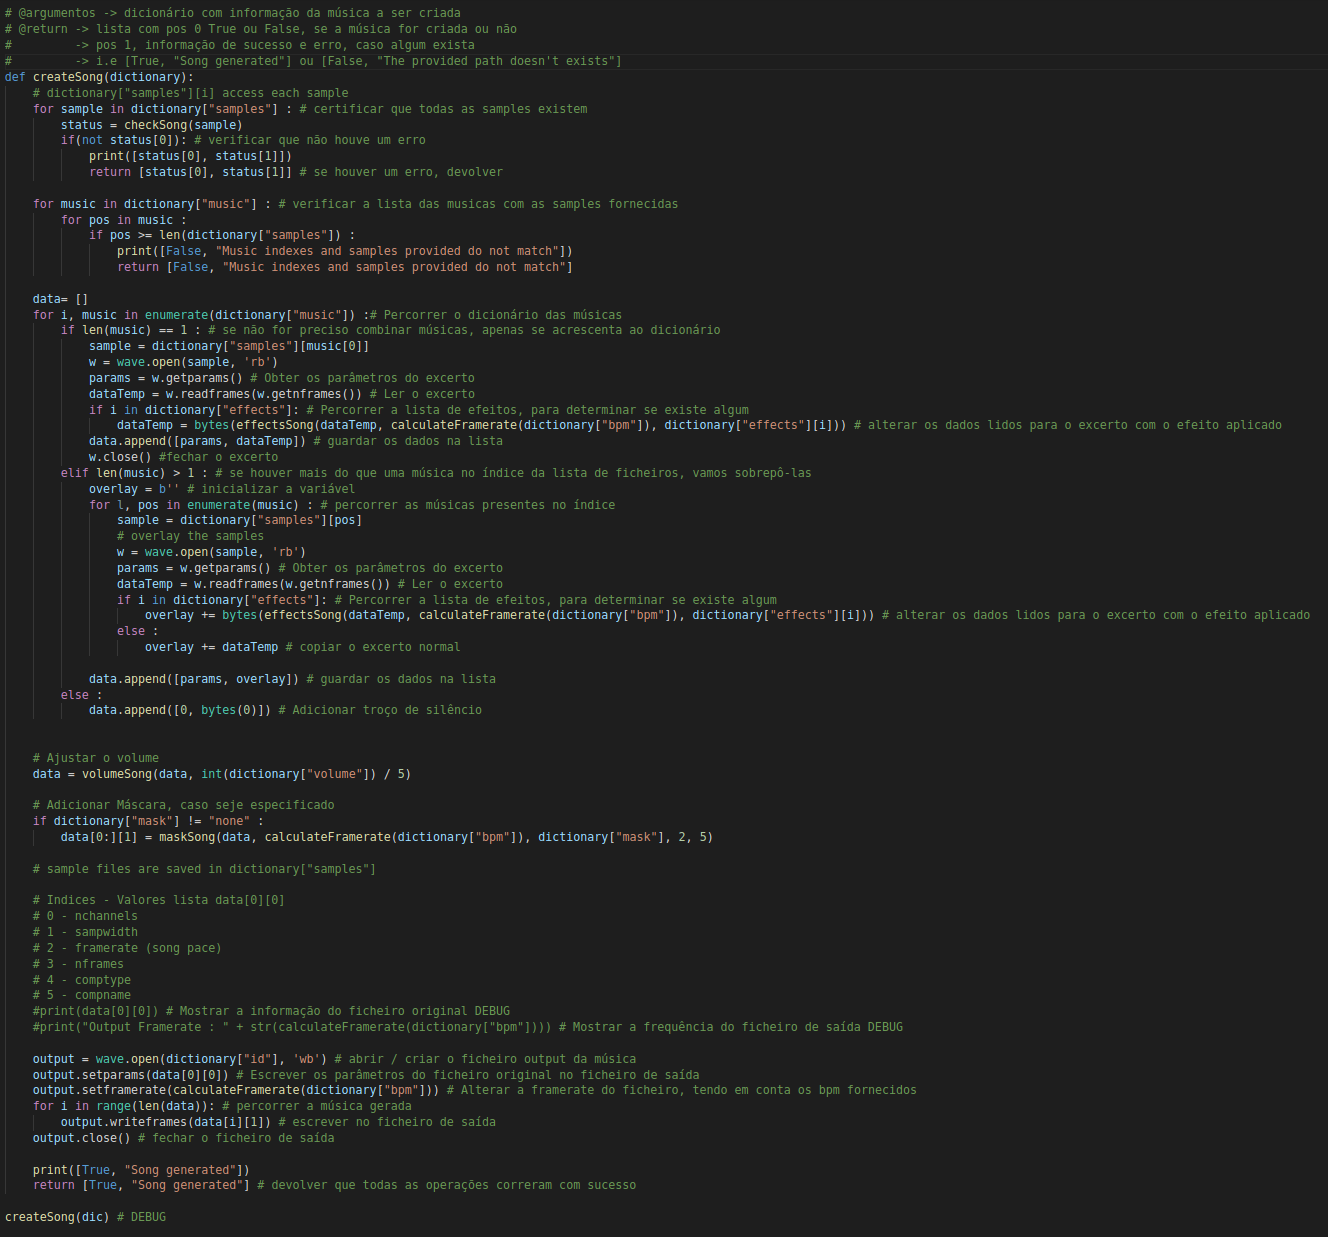
\includegraphics[width=330pt]{img/createSong.png}
\caption{Código da função createSong}
\label{fig:createSong}
\end{figure}

%%%%%%%%%%%%%%%%%%%%%%%%%%%%%%% MET: CHERRYPY %%%%%%%%%%%%%%%%%%%%%%%%%%%%%%%
\section{Servidor Cherrypy}
\label{sec:serCherrypy}
Neste secção será apresentada a metodologia do Cherrypy, ficheiro App.py.

O servidor contêm 2 funções de ajuda, funções para abrir as diversas páginas web e funções que as páginas web chamam para receber/introduzir dados da base da dados.
\subsection{Função getSample}
\label{ssec:getSample}
A função getSample é uma função de ajuda, que tem um parâmetro (id) o qual é usado para procurar um excerto.
Esta devolve o caminho do sistema de ficheiros,caso o excerto exista.
Para tal faz uma pesquisa na base de dados, se a pesquisa devolver alguma coisa então o excerto existe, caso contrário o excerto não existe então devolve None.\\
A \textbf{\autoref{fig:getSample}} mostra como isto é feito em código.

\begin{figure}[!h]
\center 
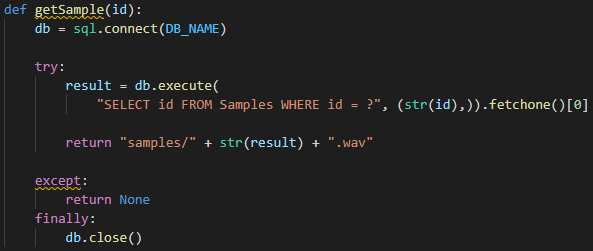
\includegraphics[width=330pt]{img/getSample.png}
\caption{Código da função getSample}
\label{fig:getSample}
\end{figure}

\subsection{Função getSong}
\label{ssec:getSong}
A função getSong é a outra função de ajuda.
Esta, tal como a anterior, tem um parâmetro (id) que é usado para procurar uma música.
O processo é exatamente igual ao da função anterior mas a pesquisa é feita na tabela Musicas em vez de ser na tabela Samples.\\
A \textbf{\autoref{fig:getSong}} mostra como isto é feito em código.
\begin{figure}[!h]
\center 
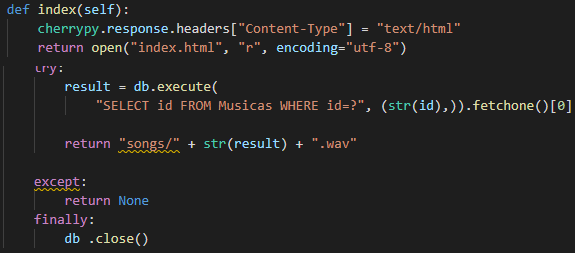
\includegraphics[width=330pt]{img/getSong.png}
\caption{Código da função getSong}
\label{fig:getSong}
\end{figure}

\subsection{Funções para abrir páginas web}
\label{ssec:abrirWebPages}
O site tem várias páginas e para navegar nelas é preciso que o servidor esteja pronto para receber os pedidos de navegação.
Para tal existem funções que devolvem a página desejada.
Como estas funções são todas iguais ou bastante parecidas, decidimos juntá-las numa secção.\\
A \textbf{\autoref{fig:index}} mostra como isto é feito em código.

\begin{figure}[!h]
\center 
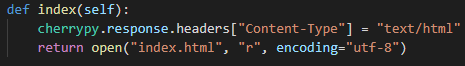
\includegraphics[width=330pt]{img/index.png}
\caption{Código da função index}
\label{fig:index}
\end{figure}

\subsection{Função list}
\label{ssec:list}
A função list devolve uma lista com músicas ou samples dependendo do que é pedido.
Para tal, esta faz uma pesquisa na base de dados e devolve a lista com os resultados.
Caso o tipo pedido não seja válido, a função devolve um dicionário a indicar que deu erro e com uma mensagem a explicar.\\
A \textbf{\autoref{fig:list}} mostra como isto é feito em código.

\begin{figure}[!h]
\center 
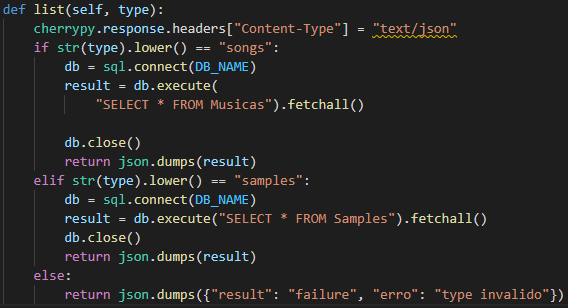
\includegraphics[width=330pt]{img/list.png}
\caption{Código da função list}
\label{fig:list}
\end{figure}

\subsection{Função get}
\label{ssec:get}
A função get devolve o caminho do sistema de ficheiros da música ou excerto.
Para tal, usa as funções de ajuda \textbf{\autoref{ssec:getSample}} e \textbf{\autoref{ssec:getSong}}. Se estas funções devolverem alguma coisa, então a música/excerto existe e o caminho deste é devolvido, caso contrário devolve um dicionário com a indicação de que falhou e uma mensagem de erro.\\
A \textbf{\autoref{fig:get}} mostra como isto é feito em código.

\begin{figure}[!h]
\center 
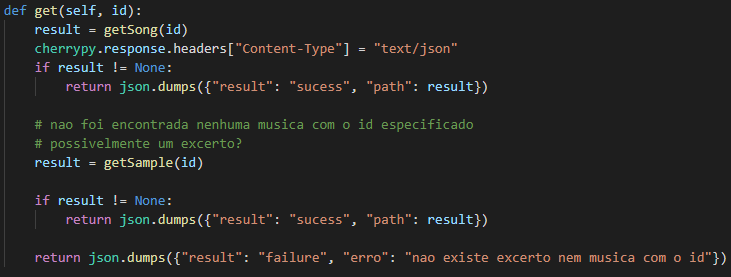
\includegraphics[width=330pt]{img/get.png}
\caption{Código da função get}
\label{fig:get}
\end{figure}

\subsection{Função put}
\label{ssec:put}
A função put gera uma música e insere a informação na base de dados.
A música gerada é baseada numa pauta criada em js numa das páginas web.\\
Devolve um dicionário a indicar o resultado da operação (sucesso ou falho) e uma mensagem de erro caso tenha falhado.\\
A \textbf{\autoref{fig:put}} mostra como isto é feito em código.

\begin{figure}[!h]
\center 
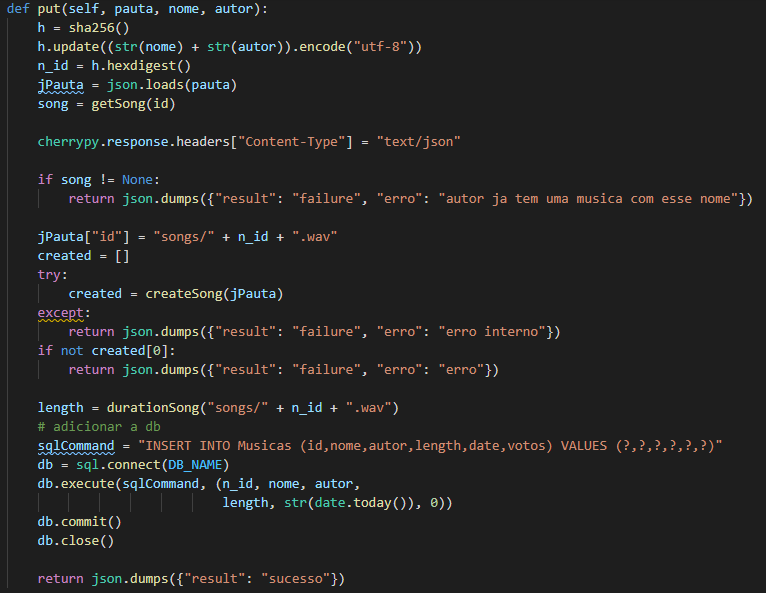
\includegraphics[width=330pt]{img/put.png}
\caption{Código da função put}
\label{fig:put}
\end{figure}

\subsection{Função uploadSample}
\label{ssec:uploadSample}
A função uploadSample deixa o utilizador introduzir um excerto no sistema, através de uma página web.
Na função, o excerto é lido e um ficheiro wav é criado com um nome (id) também gerado em código.
Os dados do ficheiro são guardados na base de dados caso o excerto tenha sido guardado com sucesso.\\
Devolve um dicionário a indicar o resultado da operação e uma mensagem de erro caso tenha falhado.\\
A \textbf{\autoref{fig:uploadSample}} mostra como isto é feito em código.

\begin{figure}[!h]
\center 
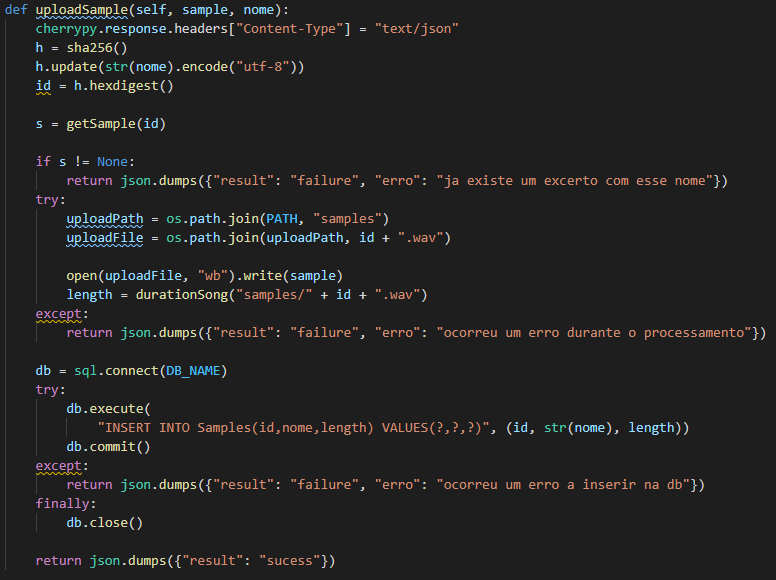
\includegraphics[width=330pt]{img/uploadSample.png}
\caption{Código da função uploadSample}
\label{fig:uploadSample}
\end{figure}

\subsection{Função vote}
\label{ssec:vote}
A função vote atualiza os votos, de uma música, na base de dados.\\
Devolve um dicionário a indicar o resultado e uma mensagem de erro caso a operação tenha falhado.\\
A \textbf{\autoref{fig:vote}} mostra como isto é feito em código.

\begin{figure}[!h]
\center 
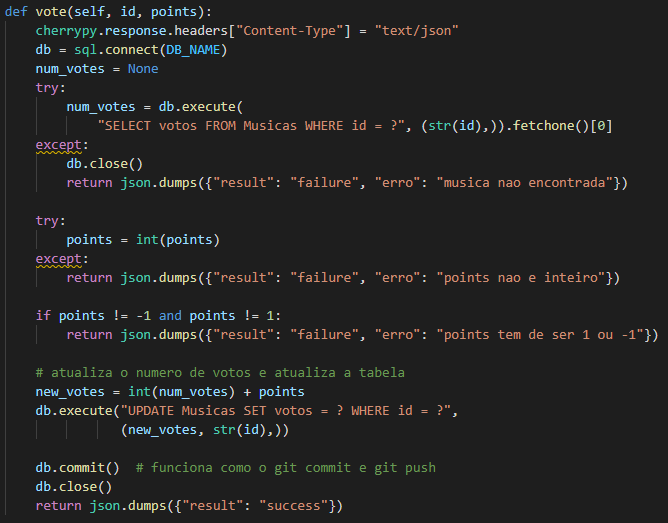
\includegraphics[width=330pt]{img/vote.png}
\caption{Código da função vote}
\label{fig:vote}
\end{figure}

%%%%%%%%%%%%%%%%%%%%%%%%%%%%%%% MET: SQL %%%%%%%%%%%%%%%%%%%%%%%%%%%%%%%
\section{SQL}
\label{sec:sql}
Para a criação da base de dados, utilizamos o terminal, usando o programa sqlite3.
Usando os comandos( CREATE TABLE Musicas();), colocando os diferentes campos com a 
respetiva indicaçao do tipo(INTEGER, TEXT, FLOAT, etc) dentro dos parênteses.
Neste caso usámos vários campos, Id para identicar a música, Nome para indicarmos 
o nome da música, Autor para sabermos a quem pertence a música, path para podermos 
armazenar e saber onde está a música, votos para podermos saber quantos votos a 
música já recebeu, length para sabermos o tamanho da música e por fim date para 
sabermos quando é que a música foi criada.
Durante a resolução do trabalho foram colocados alguns valores para as funcionalidades 
do trabalho serem testadas, para isso usámos o comando INSERT disponível no sqlite3 
(INSERT INTO Musicas VALUES();) introduzindo os valores para cada campo dentro dos 
parênteses (\textbf{\autoref{fig:tabelas_db}}).
Também criámos uma tabela Samples para guardar informação sobre os excertos.

\begin{figure}[!h]
\center 
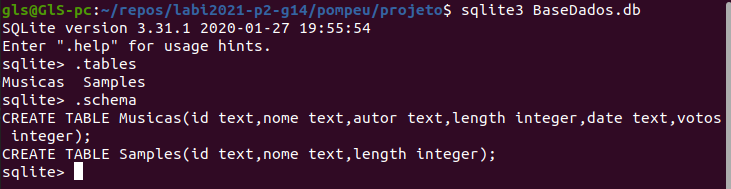
\includegraphics[width=330pt]{img/tabelas_db.png}
\caption{Tabelas da base de dados}
\label{fig:tabelas_db}
\end{figure}

%%%%%%%%%%%%%%%%%%%%%%%%%%%%%%% MET: INTERFACE WEB %%%%%%%%%%%%%%%%%%%%%%%%%%%%%%%
\section{Interface Web}
\label{sec:interfaceWeb}
\hspace{5pt}Nesta secção, será explicada a estrutura e funcionamento da Interface Web 
e o modo como comunica com o servidor.

\subsection{Página Web}
\label{ssec:paginaweb}
\hspace{5pt}A Interface  foi criada através de um template retirado da internet (Spify) \cite{spify}. 
Tal como é mencionado no enunciado, é constituída por 3 páginas, sendo a primeira a página 
onde são listadas todas as músicas da aplicação, a segunda a página onde são listados os 
excertos e a terceira a página que tem o gerador de músicas. \cite{icon} \cite{gradientetexto}

\subsubsection{Index}
\label{ssec:Index}
\hspace{5pt}A página Index sofreu algumas alterações, nomeadamente a cor de fundo, a imagem 
de overlay, a barra de navegação, alguns detalhes como títulos, o rodapé e a adição da 
funcionalidade. Foi criado um design para a aparência das músicas, com os respetivos dados: 
autor, áudio, data, dar votos e mostrar o número de votos. Esta aparência foi criada sem o 
uso de \ac{bs}, à exceção das divisões de localização deste design. \cite{icon}

\subsubsection{Samples}
\label{ssec:Samples}
\hspace{5pt}A página Samples era a antiga página "Articles" do template original. Esta página 
sofreu as mesmas alterações que a página Index, mudando apenas a funcionalidade da página. 
Para criar esta última alteração, foi criada uma tabela com a ajuda da biblioteca \ac{bs}; 
onde é possível ver o autor do excerto e o áudio deste mesmo. \cite{volslider} \cite{icon} 
\cite{audioplayer}

\subsubsection{Gerador}
\label{ssec:Gerador}
\hspace{5pt}A página Gerador era a antiga página "Privacy", sofreu as mesmas alterações que 
as restantes, à exceção da funcionalidade dessa página. Foi criada uma interface para o Gerador 
de músicas à base de \ac{bs}, onde se pode selecionar alguns parãmetros localizados nessa 
interface de maneira a ser gerada uma música com essas características. \cite{icon} \cite{audioplayer}

\subsection{JavaScript}
\label{ssec:JavaScript}
\hspace{5pt}O template já tinha algum código \ac{js} dentro de uma pasta denominada "js", o 
qual não foi alterado. Porém, foi adicionado a essa pasta 3 ficheiros: "index\_funcs, getdata 
e musicgen". Esses ficheiros são responsáveis pelas funcionalidades das 3 páginas, respetivamente. 
\paragraph{}
\hspace{5pt}O ficheiro index\_funcs tem como objetivo adicionar à página Index as funcionalidades 
correspondentes à apresentação das músicas do sistema.
Foram criadas 1 array "songs", em que cada posição correspondea  um array com informações sobre 
as músicas,  e 1 dicionário "dic" que serve de auxílio para a função que guardar os estados de 
voto quando se volta a entrar na página.

\subsubsection{Função setMusic}
\label{ssec:setMusic}
\hspace{5pt}A função setMusic tem como objetivo criar a interface que apresenta todas as opções 
descritas para a página Index. São criadas os respetivos items(div, h, span, etc...) através de 
"document.createElement("item")", adicionando as respetivas classes através de "item.classList.add("class")", 
e algumas possíveis marcas style ou outros atributos através de "item.atributo". Foi também 
estabeleciada a relação filial correta dos determinados items através de "item.appendChild(itemfilho)". 
De seguida, a última linha de código serve para estabelecer o estado dos botões de votação, sendo 
ambos falsos inicialmente porque ainda não houve votação.

\subsubsection{Funções likeUp e dislike}
\label{ssec:likeUpdislike}
\hspace{5pt}Estas funções definem em que circunstâncias é que houve uma votação positiva ou negativa. 
Ambas possuem um algoritmo muito idêntico, mudando apenas os ícones que são colocados. Na função likeUp, 
a variável like corresponde à marca "a" que é responsável pelo ícone de votação positiva. Se em dic, 
na posição 0(correspondente ao valor do voto positivo) estiver false, houve voto positivo e é criada 
a marca correspondente, sendo guardado em sessionStorage esse dado no formato \ac{json}. Caso tenha 
havido voto negativo, é executada a função correspondente(dislike). Se na posição 0 estiver true, não 
houve voto positivo e é alterado o ícone. Se não houve alteração de votos, é guardado em sessionStorage.pref 
o valor none que indica que não houve alterações. A função de dislike é praticamente igual, como referido, 
alterando apenas os ícones e as condições, que passam a corresponder ao voto negativo (\textbf{\autoref{fig:likeUp}}).

\begin{figure}[!h]
\center 
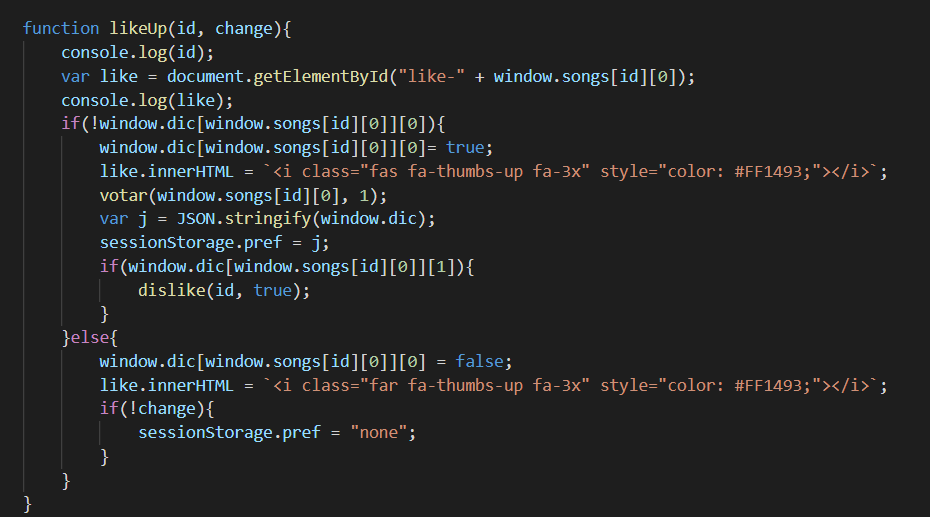
\includegraphics[width=330pt]{img/Funcao_likeUp.png}
\caption{Código da função likeUp}
\label{fig:likeUp}
\end{figure}

\subsubsection{Função loadPref}
\label{ssec:loadPref}
\hspace{5pt}Para que os votos do utilizador sejam guardados na aplicação, sem que sejam perdidos caso o 
utilizador saia desta, é necessária que haja algum mecanismo para ser feito o que foi descrito, neste 
caso é loadPref. Se não houve alterações de votação, não é feito nada. Caso tenha havido alterações de 
votação, são analizadas essas alterações e, no caso da existência de voto positivo, é executada a função 
likeUp e é executada a função dislike no caso do voto negativo \textbf{\autoref{fig:loadPref}}.

\begin{figure}[!h]
\center 
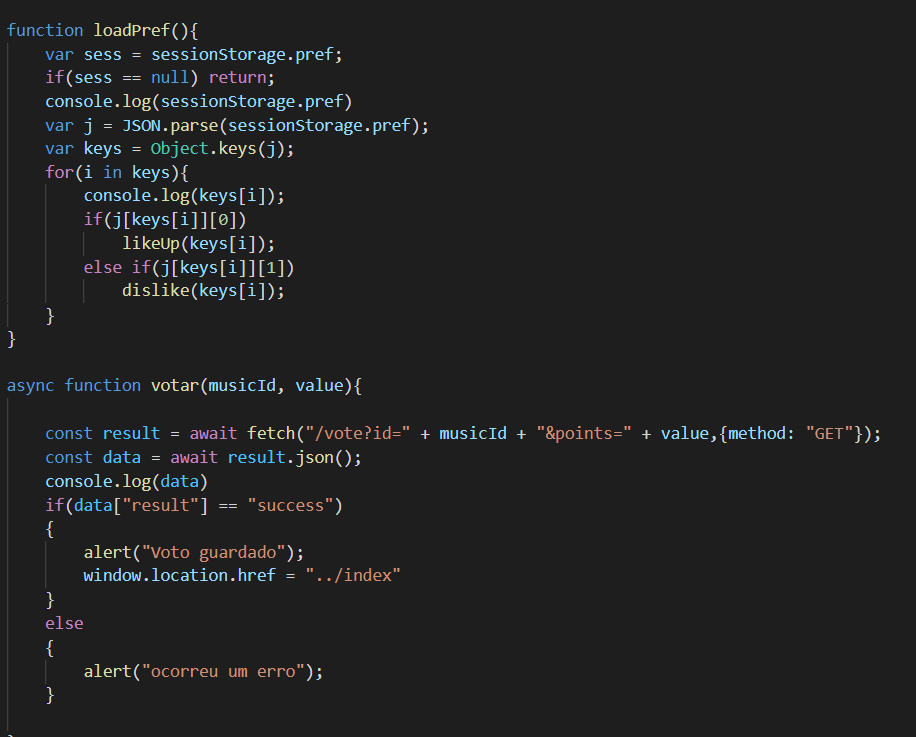
\includegraphics[width=330pt]{img/loadPrefVotar.png}
\caption{Código da função loadPref e Votar}
\label{fig:loadPref}
\end{figure}

\subsubsection{Função getMusic}
\label{ssec:getMusic}
\hspace{5pt}Esta função é a principal e obtem os dados pertencentes ao servidor e executa também as 
restantes funções. A constante result e a constante data guardam esses dados no formato \ac{json} para 
poderem ser manipulados. A variável songs vai guardar os valores em data. Logo a seguir, são executadas 
as funções setMusic e loadPref.

\paragraph{}

\hspace{5pt}O ficheiro getdata tem como objetivo adicionar à página Excertos as funcionalidades 
correspondentes à apresentação dos excertos do sistema.

\subsubsection{userAction}
\label{ssec:userAction}
\hspace{5pt}Esta função tem como objetivo realizar todas as funcionalidades da responsabilidade de 
getdata.js. Para isso, é criado, à semelhança de getMusic, uma constante response possui os dados 
do servido, que são convertidos para \ac{json} e guardados em myJson. A constante sampArr vai 
guardar o valor da chave samples proveniente de myJson, que contem os excertos. A contante tbl 
corresponde à tabela que se encontra na página. De seguida, serão criadas as várias interfaces de cada 
música existente. A constante name indica o nome da música e encontra-se na chave nome do dicionário da 
determinada posição do array sampArr. Será criada uma marca table row (tr) e as suas 2 células, que são a 
que indicará o nome do autor do excerto e o excerto em si. Por fim, é estabelecida a relação filial entre 
estas marcas e a tabela (tbl) (\textbf{\autoref{fig:userAction}}).

\begin{figure}[!h]
\center 
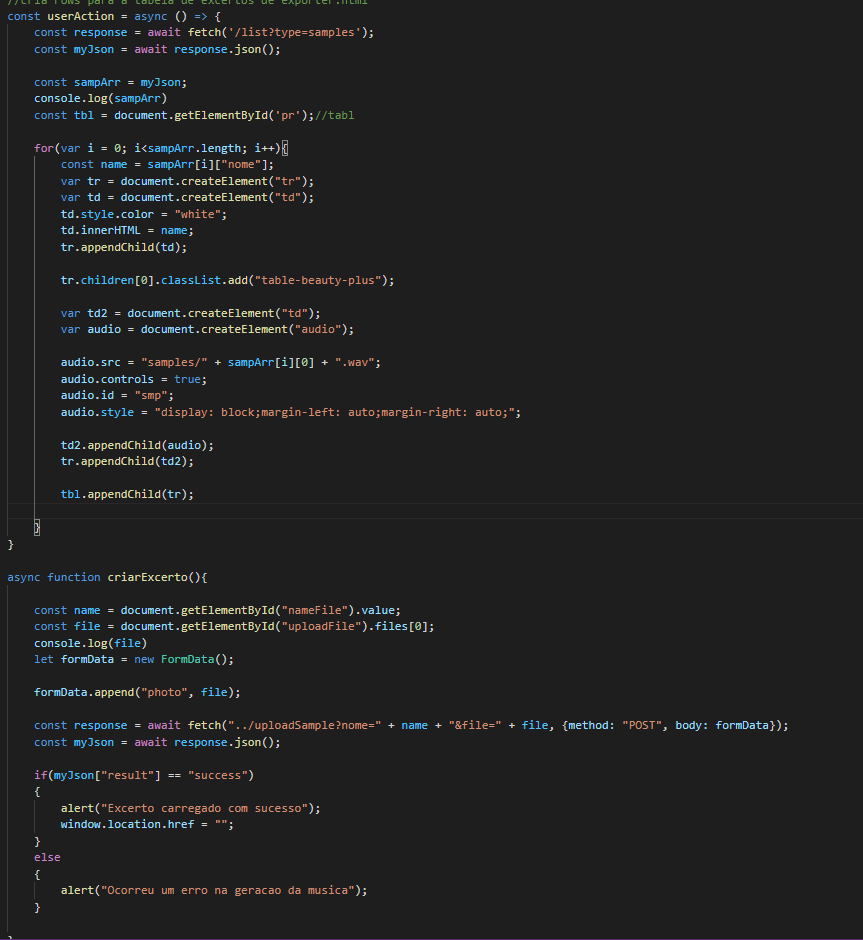
\includegraphics[width=330pt]{img/getdata.png}
\caption{Código do ficheiro getData.js, que inclui a função userAction}
\label{fig:userAction}
\end{figure}

\paragraph{}

Por fim, resta-nos explicar o ficheiro musicGen. Este ficheiro tem como objetivo gerar a interface gráfica 
do gerador de músicas correspondente à página Gerador do site.

\subsubsection{Função generateLines}
\label{ssec:generateLines}
\hspace{5pt}De acordo com o meu colega, Esta função tem como objetivo criar a tabela dinâmica da interface 
do gerador de músicas, Será criada uma tabela com as respetivas marcas, as suas classes (\ac{bs}) e é 
estabelecida a filiação respetiva.

\subsubsection{Função getSampleList}
\label{ssec:getSampleList}
\hspace{5pt}Esta função fornece os excertos necessários ao gerador de músicas. A constante response vai 
guardar os excertos provenientes do servidor e a constante myJson vai guardar os dados de response no formato 
\ac{json}, com o objetido de serem fornecidas as samples para posteriormente executar a função generateLines.

\subsubsection{Função gerarArray}
\label{ssec:gerarArray}
\hspace{5pt} A função gerarArray transforma as checkboxes num array em que cada posição contem um array com 
as opções de cada checkbox (\textbf{\autoref{fig:gerarArray}}). \cite{checkboxes}

\begin{figure}[!h]
\center 
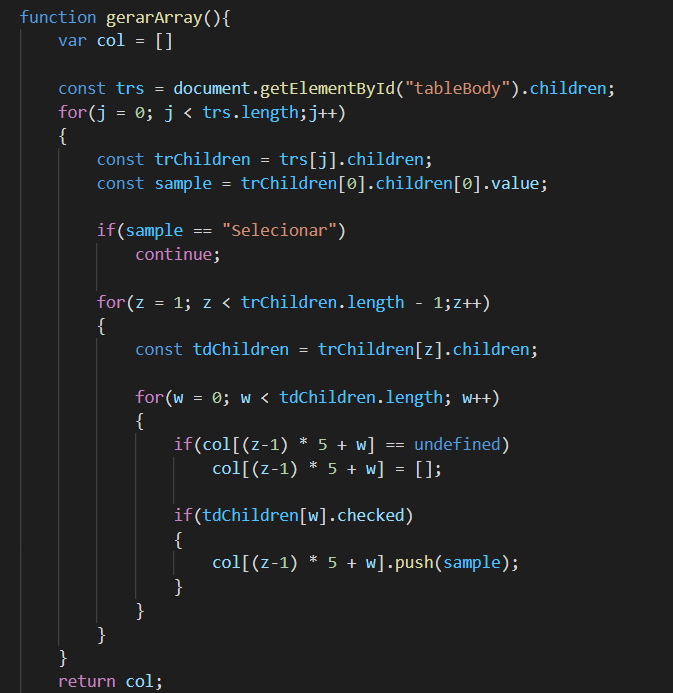
\includegraphics[width=330pt]{img/Funcao_gerarArray.png}
\caption{Código da função gerarArray}
\label{fig:gerarArray}
\end{figure}

\subsubsection{Função getEffects}
\label{ssec:getEffects}
\hspace{5pt}Esta função fornece um array com os efeitos aplicados em cada uma das linhas. Se uma linha não 
possuir efeitos, o array não vai introduzir nada na posição correspondente a essa linha.

\subsubsection{Função getSamplesWithPath}
\label{ssec:getSamplesWithPath}
\hspace{5pt}Esta função cria um array com os caminhos dos excertos para serem utilizados no servidor para 
gerar a música.

\subsubsection{Função gerar}
\label{ssec:gerar}
\hspace{5pt}Esta função envia os dados necessários para o servidor gerar uma música e avisa logo de seguida 
se essa ação foi sucedida ou não. São criadas constantes correspondentes aos variados dados (volume, \ac{bpm}, 
efeitos, etc...), para além do array com as opções das checkboxes(é chamada a função gerarArray), dos efeitos e 
dos excertos (são executadas as funções gerarArray, geteffects e getSamplesWithPath, respetivamente, para estes 
3 últimos). Estes dados são guardados numa constante, convertidos para \ac{json} e enviados neste formato para 
o servidor (\textbf{\autoref{fig:gerar}}). 

\begin{figure}[!h]
\center 
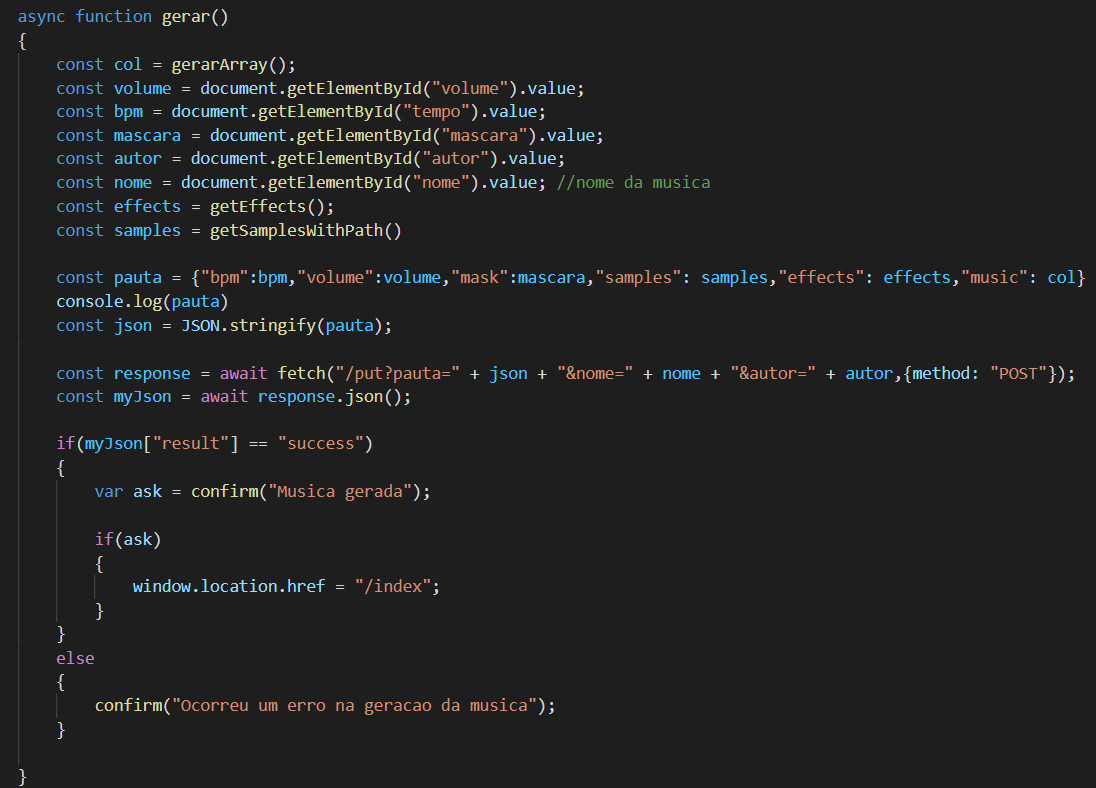
\includegraphics[width=330pt]{img/Funcao_gerar.png}
\caption{Código da função gerar}
\label{fig:gerar}
\end{figure}

%%%%%%%%%%%%%%%%%%%%%%%%%%%%%%% MET: GIT %%%%%%%%%%%%%%%%%%%%%%%%%%%%%%%
\section{Git}
\label{sec:git}
As funcionalidades do git foram muito utilizados neste projeto, desde a simples sincronização 
de ficheiros e código, até à criação, junção e gestão de branches (\textbf{\autoref{fig:git_c}} e 
\textbf{\autoref{fig:git_d}}). 
\cite{git}

\begin{figure}[!h]
\center 
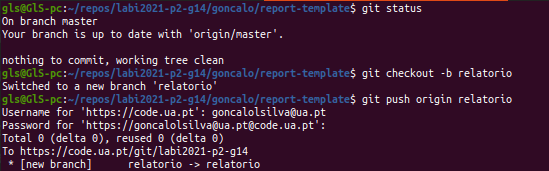
\includegraphics[height=100pt]{img/git_1.png}
\caption{Exemplo da criação de branches (criação branch relatorio)}
\label{fig:git_c}
\end{figure}

\begin{figure}[!h]
\center 
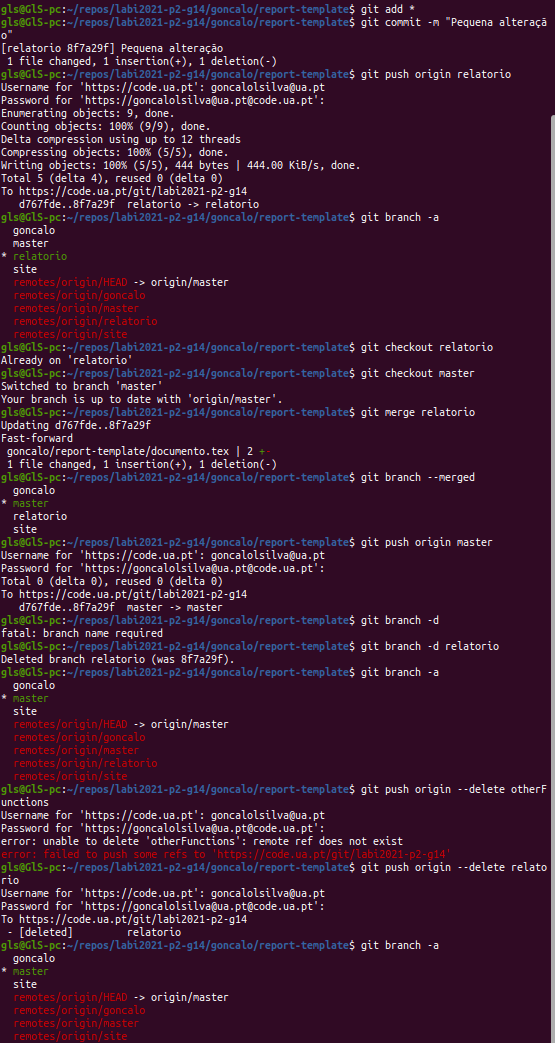
\includegraphics[height=300pt]{img/git_2.png}
\caption{Exemplo da eliminação de branches (eliminação branch relatorio)}
\label{fig:git_d}
\end{figure}

%%%%%%%%%%%%%%%%%%%%%%%%%%%%%%% MET: CODEUA %%%%%%%%%%%%%%%%%%%%%%%%%%%%%%%
\section{Code UA}
\label{sec:codeua}
As funcionalidades do Code UA forneceram bastante ajuda ao desenvolvimento do projeto, 
desde a própria visualização dos branches disponíveis, bem como a própria gestão e 
visualização do código, até à criação de funcionalidades a serem desenvolvidas e bugs 
a serem resolvidos. Pode visualizar o projeto no Code UA, através do 
link: http://code.ua.pt/projects/labi2021-p2-g14
\cite{codeua}

%%%%%%%%%%%%%%%%%%%%%%%%%%%%%%%%% RESULTADOS %%%%%%%%%%%%%%%%%%%%%%%%%%%%%%%%%

\chapter{Resultados}
\label{chap.resultados}
Descreve os resultados obtidos com este relatório.

\section{Funcionamento}
\label{sec:funcionamento}

A \autoref{fig:iniciar_server} mostra o comando de inicio do servidor.
Mostrar o servidor em funcionamento

\section{Testes}
\label{sec:testes}

Os testes às funcionalidades foram feitos através de testes funcionais e unitários criados para 
o efeito. Estes testes são corridos usando a ferramenta pytest incorporada no python. 
Os testes albergam três ficheiros, o ficheiro test\_songEngine.py e test\_func\_songEngine.py, 
testam as funções de criação e obtenção de músicas do servidor, através de testes unitários e
funcionais. O ficheiro test\_app.py, testa as funcionalidadesdo servidor cherrypy.

É possível correr estes testes através do comando \textbf{"python3 -m pytest"}, como nos mostra 
a \autoref{fig:testes}.

\begin{figure}[ht]
\center 
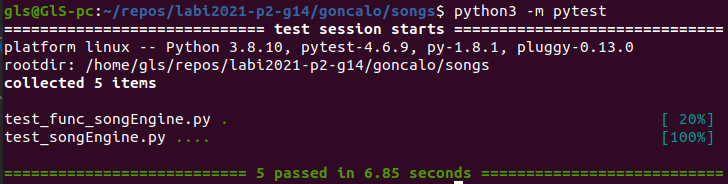
\includegraphics[height=90pt]{img/pytest.png}
\caption{Exemplo de execução dos testes ao songEngine}
\label{fig:testes}
\end{figure}

%%%%%%%%%%%%%%%%%%%%%%%%%%%%%%%%% ANÁLISE %%%%%%%%%%%%%%%%%%%%%%%%%%%%%%%%%

\chapter{Análise}
\label{chap.analise}
Analisa os resultados.
Mostrar que as músicas foram criadas e ficou tudo correto

%%%%%%%%%%%%%%%%%%%%%%%%%%%%%%%%% CONCLUSÕES %%%%%%%%%%%%%%%%%%%%%%%%%%%%%%%%%
\chapter{Conclusões}
\label{chap.conclusao}
Com este trabalho, conseguimos solidificar o nosso conhecimento em várias linguagens, como HTML, JavaScript, CSS e 
Python, bem como outras funcionalidades, como o cherrypy, pytest e operações com músicas (wave) \cite{stackoverflow}
 \cite{schools} \cite{librariabootstrap}.
Apesar das adversidades, acreditamos que o trabalho foi conseguido com sucesso, criámos uma aplicação 
web com as funcionalidades referidas e todas as características necessárias para tal, utilizando os recursos que 
nos foram fornecidos e auxiliando a sua compreensão com este relatório.

\chapter*{Contribuições dos autores}
O \ac{pc} desenvolveu o servidor Cherrypy, bem como os testes para o mesmo. Ajudou o \ac{st} e \ac{gs} no código
de conexão backend e em outros assuntos. Também fez a secção acerca do servidor Cherrypy neste relatório, bem como
parte da SQL, visto que este desenvolveu parte do código da mesma.
O \ac{gs} desenvolveu o songEngine, bem como os testes para o mesmo. Ajudou um pouco \ac{st} no código frontend e backend,
nomeadamente, na terceira página. Além disso, também começou este relatório e fez a secção acerca do songEngine, bem como os
capítulos Introdução, Resumo, Agradecimentos, Conclusão, e a subsecção CodeUa e GIT. 
O \ac{st} editou o template e fez o código html base para o site, bem como as páginas e código backend, 
tendo ficado responsável pela Interface Web e pela escrita da mesma secção neste relatório.
O \ac{hh} criou a base de dados inicial e escreveu parte da secção de SQL do relatório.
O \ac{gs} fez 34\% do trabalho, o \% \ac{pc} fez 34\% do trabalho, o \ac{st} fez 27\% e o \ac{hh} fez 5 \% do trabalho.

%%%%%%%%%%%%%%%%%%%%%%%%%%%%%%%%% ACRÓNIMOS %%%%%%%%%%%%%%%%%%%%%%%%%%%%%%%%
\chapter*{Acrónimos}
\begin{acronym}
\acro{ua}[UA]{Universidade de Aveiro}
\acro{miect}[MIECT]{Mestrado Integrado em Engenharia de Computadores e Telemática}
\acro{lei}[LEI]{Licenciatura em Engenharia Informática}
\acro{labi}[LABI]{Laboratórios de Informática}
\acro{bpm}[BPM]{Beats Per Minute}
\acro{glisc}[GLISC]{Grey Literature International Steering Committee}
\acro{js}[JS]{JavaScript}
\acro{bs}[BS]{Twitter Bootstrap}
\acro{json}[JSON]{JavaScript Objective Notation}
\acro{gs}[GS]{Gonçalo Silva}
\acro{pc}[PC]{Pompeu Costa}
\acro{st}[ST]{Samuel Teixeira}
\acro{hh}[HH]{Hugo Hadden}
\end{acronym}


%%%%%%%%%%%%%%%%%%%%%%%%%%%%%%%%% BIBLIOGRAFIA %%%%%%%%%%%%%%%%%%%%%%%%%%%%%%%%
\printbibliography

\end{document}
